\chapter{Method}

This chapter will introduce and develop the \rrtfunnel\ algorithm, through two
means: Developing robust motion primitives through the \ac{SOS} programming
framework, based on the work in~\cite{majumdarFunnelLibrariesRealtime2017}, and
second deploy these funnels as motion primitives in a discrete \ac{RRT} planner,
based on~\cite{lavalleLav98cPdf}. This is beneficial, as using \textit{robust}
motion primitives has several advantages. Firstly, they are robust to
uncertainty, and thus, as long as the uncertainties in the system are akin to
our assumptions, the vehicle will not leave the funnel path. Secondly, with the
assumption that the primitives are robust, there is no need for more
conservative maneuvers and heuristics, such as maximizing the distance to an
obstacle. This means that a robust motion primitive algorithm can perform more
aggressive maneuvers than one that is inherently cautious about its
environment~\cite{majumdarFunnelLibrariesRealtime2017}.

\section{The funnel part}

In order to create a basic set of funnels as the robust motion primitives for
the \rrtfunnel{} motion planning algorithm, a few obstacles have to be overcome
first. The first one is settling on a model for the funnel calculations. After a
little bit back and forth, the simple car model from \cite[LaValle.p~613]{Lav06} was
chosen and slightly modified into
\begin{equation}
  \label{eq:model-dynamics}
  \mathbf{x} =
  \begin{bmatrix}
    x \\ y \\ \theta \\ \dot{\theta} \\
  \end{bmatrix}, \,
  \dot{\mathbf{x}}  =
  \begin{bmatrix}
    -v(t)\sin(\theta) \\
    v(t)\cos(\theta) \\
    \dot{\theta} \\
    u \\
  \end{bmatrix},
\end{equation}
which is a second-order unicycle model with constant speed. A picture of the
model can be found in figure~(\ref{fig:second-order-unicycle}).

\begin{figure}
  \centering
  \resizebox{10em}{!}{
    \import{figures/method/}{unicycle-model.pdf_tex}
  }
  \caption{The unicycle model of a vehicle.}
  \label{fig:second-order-unicycle}
\end{figure} 

Although this is the only model used in this thesis, the framework and the code
is easily adapted into accommodating a different and more complicated model for
planning.


\subsubsection{Generating the trajectories}

The trajectories are generated through the \textit{Direct collocation method}.

Using a cost function of the type
\begin{equation}
  J = \int_{0}^{T} \left[ 1 + {u_{0}}^{T}Ru_{0} \right] dt
\end{equation}

The initial trajectory set is pictured in~\ref{fig:initial-trajectories}, and
consists of a left-turn, a straight-forward, and a right-turn motion.

\begin{figure}
  \centering
  \begin{minipage}[b]{0.4\textwidth}
    \includegraphics[width=\textwidth]{figures/method/straight-trajector}
  \end{minipage}
  \hfill
  \begin{minipage}[b]{0.4\textwidth}
    \includegraphics[width=\textwidth]{figures/method/left-trajector}
  \end{minipage}
  \hfill
  \begin{minipage}[b]{0.4\textwidth}
    \includegraphics[width=\textwidth]{figures/method/right-trajector}
  \end{minipage}
  \caption{The three motion primitives for the \rrtfunnel{} algorithm, one
    straight, one left, and one right turn.}
  \label{fig:initial-trajectories}
\end{figure}


\subsubsection{Initializing the funnel calculations with a TVLQR candidate as
  the initial Lyapunov function}

The funnel calculation algorithm has to be initialized with a Lyapunov
candidate. Just like in the paper~\cite{majumdarFunnelLibrariesRealtime2017},
funnels will be initialized with a \ac{TV-LQR} controller. The
\ac{LQR}-controller has a cost function of the form
\begin{equation}
  J = x^{T}(t_1)F(t_1)x + \int_{t_{0}}^{t_{1}} \left( x^{T}Qx + u^{T}Ru + 2x^TNu \right) \mathrm{d}t,
\end{equation}
which when employed on the linearization of the system dynamics
\begin{equation}
  \dot{\bar{x}} \approx A(t)\bar{x}(t) + B(t)\bar{u}(t) +D(t)w(t),
\end{equation}
gives an initial candidate Lyapunov function
\begin{equation}
  V(t,x) = {\bar{x}}^{T}S_{i}\bar{x}.
\end{equation}

Although the focus of this thesis is not on fine-tuning the controller, some
amount of effort has to go into getting the cost parameters acceptable. In
general penalizing the vehicle's distance from the nominal path in
\((x,y,\theta)\), and not caring for the energy expended, the control input will
be penalized very little. More specifically the cost matrices employed are
\begin{align*}
  R &= 0.01 \\
  Q &= \begin{bmatrix}
    40 & 0 & 0 & 0 \\
    0 & 40 & 0 & 0 \\
    0 & 0 & 0 & 40 \\
    0 & 0 & 0 & 4 \\
  \end{bmatrix}
  \\
  Q_{f} &= 2*\mathrm{diag}(2, 1.5, 1, 1) \\
\end{align*}
where the control input is only penalized \(\frac{1}{10}\)th of the other variables.

Tuning of the LQR paramaeters, and why the costs were chosen!

\subsubsection{Generating the funnels around the trajectories}

With the nominal trajectories, and the initial Lyapunov functions now ready, the
funnels around the nominal trajectories can be calculated using the
algorithm~\ref{alg:funnelalgorithm}. The implementation is an expansion upon
code from the~\cite[Drake toolbox]{drake}, whereas the \ac{SOS} implementation
is kicked out to a \ac{SOS} solver built upon~\[sostools\]\cite{sostools}.

First of all the system dynamics for the model~\ref{eq:model-dynamics} are still
not polynomial, so the polynomial system needed for the \ac{SOS}-verification is
obtained through a Taylor-expansion of degree three around the nominal
trajectory.

Secondly the function limiting the size of the funnel \(\rho(t_{k})\) has to be
initialized by a feasible \(\rho(t)\) as well. This is done through the equation
\begin{equation}
  \rho(t_{k}) = \mathrm{exp}\left( \rho_{\tau}\frac{\left( t_{f} - t \right)}{\left( t_{f} - t_{0}  \right)}\right)
\end{equation}
from~\cite[eq.~6.sec~3]{tobenkinInvariantFunnelsTrajectories2010}. Where
\(\rho_{\tau}\) is a positive constant determining the ubber bound on the
funnel. If the given choice of \(\rho_{\tau}\) does not verify a funnel, either
increase the value of \(\rho_{\tau}\), and optionally the number of sampled
points from the trajectory to be
verified~\cite{tobenkinInvariantFunnelsTrajectories2010}.

Thirdly, the initial condition set has to be decided beforehand. In general the
initial condition set can be any semi-algebraic set in the state-space. However,
a simple way of obtaining a initial condition set for the trajectories at hand
is by taking advantage of the Lyapunov function canditate from the
\ac{LQR}-controller. Thus by setting
\begin{equation}
  \mathcal{X}_{0} = \frac{S_{k}}{\rho_{\tau}}
\end{equation}
an intial condition is obtained. For the controller 

For the cost function in the funnel generation
algorithm~\ref{alg:funnelalgorithm}, which in general is a maximization of the
determinant of the upper bound ellipse for the funnel set, a weight is added to
each element in order to further fine-tune the size of the funnel. As an example: For the
vehicle model in this thesis the size of the funnel projected down into the
xy-plane will be the most important metric. Whether or not the vehicle's
orientation parameter \(\theta\) is  close to the nominal heading is of less
concern, and is therefore down-prioritized, along with the cost on the control
input \(u\). Having a large \(theta\) and \(\dot{\theta}\) semi-axis in the
hyperellipsoid can also be beneficial, as it increases the inlet of the funnel
at hand. This leads to the cost function
\begin{equation}
  P_{k} = W_{k}P_{k}W_{k}^{T}
\end{equation}
where
\begin{equation}
  W_{k} =
  \begin{bmatrix}
    10 & 0 & 0 & 0 \\
    0 & 10 & 0 & 0 \\
    0 & 0 & 1 & 0 \\
    0 & 0 & 0 & .1 \\
  \end{bmatrix}
\end{equation}

Initially the modified cost function
from~\cite{majumdarFunnelLibrariesRealtime2017} was added, but the 

Plot figures with different weightings of the cost functions.

Running the funnel calculations with the plots of the funnels generated.

Funnels with different degree LaGrangian multipliers.

Funnels with different sampling density?

Funnels with different cost functions.

Funnels with 

\subsubsection{Adding uncertainty to the Funnels}

The initial code in the~\cite[Drake toolbox]{drake} did not take uncertainty
into account, and hence had to be added to the implementation.

When adding uncertainty to the speed of the vehicle, so that the speed is now in
\([9,11]\) m/s.

Adding uncertainty to the speed where the uncertainty was greater than or equal
to two, neither of the three motion primitives were verified using the program.


\subsubsection{Expanding the funnels with the size of the vehicle model}

In order for the funnel to be valid, it needs to be expanded from the point
model used, to contain the entire vehicle in it's \ac{ROA}. This is done through
expanding the size of the funnel by the radius of the vehicle, and can be seen
in~(\ref{fig:expanded-funnel}).

\begin{figure}
\centering
\includegraphics[clip, trim=6cm 8cm 6cm 8cm, scale=.5]{figures/method/expanded-funnel}
\caption{The original funnel created from the point model, with a funnel
  expanded by a radius of 0.2 surrounding it.(TODO)- maybe draw this in inkscape
instead?}
\label{fig:expanded-funnel}
\end{figure}

\subsubsection{Shifting funnels and invariance}

In order to freely shift funnels around in the configuration space, the cyclic
coordinates of the system has to be determined. ex:
\begin{align}
  \mathcal{L} &= T - V = \frac{1}{2} mv^2 + \frac{1}{2}I\dot{\theta}^2 \\ 
              &= \frac{1}{2} 
                m\begin{bmatrix}
                  -v\sin \theta \\ 
                  v \cos \theta \\
                  \dot{\theta} \\
                  u \\
              \end{bmatrix}^{T} 
  \begin{bmatrix}
                  -v\sin \theta \\ 
                  v \cos \theta \\
                  \dot{\theta} \\
                  u \\
                \end{bmatrix}
  - I\dot{\theta}^2 \\
              &= m \left(
                v^2 \sin^2 \theta + v^2 \cos^2 \theta + {\dot{\theta}}^2 + u^2
                \right)  + I {\dot{\theta}}^2 \\
              &= m(v^2 + {\dot{\theta}}^2 + u^2) + I {\dot{\theta}}^2 \\
\end{align}
which shows that the LaGrangian is invariant to shifts in the \((x,y,\theta)\)
variables. 

\subsection{Checking which funnels can be composed and not}

If two funnels are composable as per definition~(\ref{def:funnel-composition}),
then it is safe to build one as a motion primitive on top of the other. This
definition can be translated into a \ac{SOS}-program, to ensure that the outlet
of one funnel is fully contained in the outlet of the other.

\subsection{The Identity funnel}

\subsection{Simulating the funnels, checking if the model stays within the
  funnel at all times.}

\section{Distance metric for expansion (Maybe for the RRT section?)}

\section{RRT}

\subsection{Rapidly exploring the state-space}

One of the attributes of an \ac{RRT} is it's ability to quickly expand deep into
the search-space, and later on start the finer search TODO - cite. In order to
enable this behaviour for the \rrtfunnel{} algorithm, a couple of longer motion
primitives are needed. These are easily built by composing several of the longer
primitives from the base set. Still, they will not be made infinitely long,
which adds the familiar constraint of.. TODO - cite.

\subsubsection{The identity funnel for starting the simulation fresh}

The identity funnel is an empty placeholder for the start node of the graph,
that does no transformations on the model at all, and thus can be seen as the
identity element in the funnel space, or rather, the identity funnel.

\section{FunnelGraph}

One can think of funnels computed using the machinery described in
\cite[sec~4]{majumdarFunnelLibrariesRealtime2017} as \textit{robust} motion
primitives~\cite{majumdarFunnelLibrariesRealtime2017}.

As every subfunnel (\ie{} part of a funnel), is also a funnel, funnels can be
pruned. Therefore, cutting off the end, or the beginning of a funnel, will in
fact create two new funnels. This fact can be exploited in order to create new
and shorter subfunnels for use in the \rrtfunnel{} algorithm.

\begin{figure}
  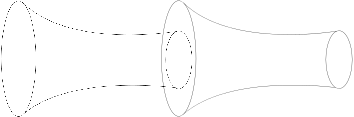
\includegraphics[scale=.2]{figures/method/funnel-composition}
  \centering
  \caption{Two funnels composed.}
\end{figure}

Look at ~\cite{vonasekGlobalMotionPlanning2013} (Algorithm3) for a way of
building an RRT with motion primitives.

\subsection{Composition of funnels}

In order to ensure that the motion primitives in the \ac{RRT} can be added onto
eachother, and that this addition does not remove the robustness guarantess
embroidered in a single funnel. Thus in order to ensure that two motion
primitives are composable.

\section{TVLQR}

Tuning of the parameters in the \textit{TVLQR} algorithm.

\section{Simulations}

\subsection{Collision checking}

\subsection{Staying inside the funnels}

As a funnel is not simply the 2D-ellipse projected down into the plane. In fact
the funnel lives in 4D space, and as such the vehicle can leave the funnel, even
though it is inside the projected funnel in 2D space. Therefore the \rrtfunnel{}
algorithm checks at each step during the simulations that the vehicle stays
inside the verified funnels. This is done through inputting the vehicle's
current state into the quadratic Lyapunov function
\[
  {\bar{x}}^{T}S_{k}\bar{x} + \bar{x}s_{1} \bar{x} s_{2}
\]

\section{Creating more motion primitives}

Although the base motion primitive library is pretty sparse, just like the
\rrtfunnel{} algorithm creates paths from stacking motion primitives, longer
motion primitives can be built \textit{for} the \rrtfunnel{} algorithm. This is
beneficial also, as it helps the algorithm expand quickly into the unsearched
parts of the searchspace, and therefore helps it regain some of the benefits of
the original \ac{RRT} algorithm.

(Downsides -- does not necessarily expand into other parts than the xy-plane?).

A collection of the added motion primitives is shown in~(\ref{fig:expanded-motion-primitives}).

\begin{figure}
  % \includegraphics[scale=.5]{figures/method/expanded-motion-primitives}
  \caption{A collection of motion primitives built from the base set of
    primitives.}
  \label{fig:expanded-motion-primitives}
\end{figure}

\subsection{}

\section{Funnel-graph}

Even though the \rrtfunnel{} algorithm can work just fine with a collection of
funnels, and simply bruteforcing all funnels at the planning stage, it is
helpful to associate some kind of structure with the collection. In essence
associating the collection of funnels \(\mathcal{F}\) with some structure.
Giving the collection \(\mathcal{F}\) a tree structure, where each node in the
tree is reached, either through a funnel, a part of a funnel (which is also a
funnel), or a composition of funnels. Each funnel already has a set of nodes
associated with itself from the discretization taking place prior to funnel
creation as shown in figure \ref{fig:somefig}.

\begin{figure}
  \centering
  \begin{minipage}[b]{0.4\textwidth}
    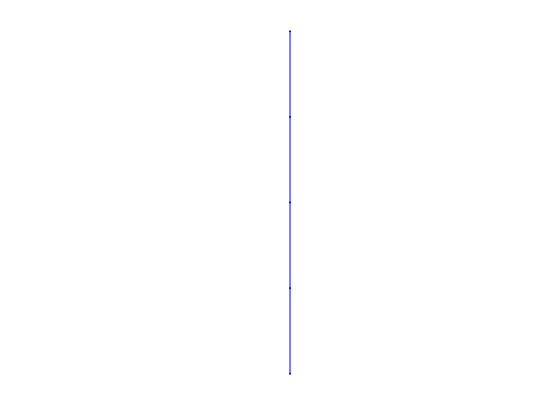
\includegraphics[width=\textwidth]{figures/method/trajectory-sampled}
    \caption{Trajectory sampled \# times (TODO)}
  \end{minipage}
  \hfill
  \begin{minipage}[b]{0.4\textwidth}
    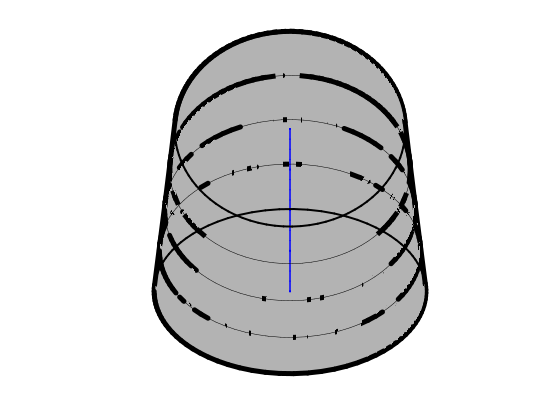
\includegraphics[width=\textwidth]{figures/method/funnel-sampled}
    \caption{The verified trajectory ellipsis overlaid at the sample times.}
  \end{minipage}
\end{figure}

For each funnel, in order to not only be able to compose funnels, but
sub-funnels, which means that at every point of every node in every funnel
composability with every other sample point in every other funnel has to be
checked. This is summed up more orderly in algorithm
\ref{alg:create-funnel-graph}, where a funnel is a vertice in the graph, and an
ordered pair of funnels \(\left( F_{i}, F_{j} \right)\) is an edge. Composition
of funnels is checked in the same way as in \ref{def:funnel-composition}.

\begin{algorithm}
  \caption{Create Funnel Graph}
  \label{alg:create-funnel-graph}
  \DontPrintSemicolon \SetAlgoNoLine

  \KwIn{\(\mathcal{F}\) -- The basis set of funnels computed around the nominal
    trajectories.} \KwOut{\(\mathcal{G}(\mathcal{F})\) -- Directed graph
    representing the composability of funnels.}

  \ForEach{\(F_{i} \in \mathcal{F}\)} { \ForEach{\(F_{j} \in \mathcal{F}\)} {
      \ForEach{\(t_{k} \in F_{i}\)} { \ForEach{\(t_{l} \in F_{j}\)} {
          \If{\(F_{i}(t_{k}) \subset F_{j}(t_{l})\)} { \(\mathcal{G}
            \leftarrow{} \left( F_{i}(t_{k}), F_{j}(t_{l}) \right)\) } \; } \; }
      \; }\; }\;

\end{algorithm}

Hereafter the primities at each point can be prioritized by some metric, say
distance to the goal or similar.

\subsection{Verify that the vehicle stays within the funnels}

Below is a figure of N simulation runs with the model vehicle in all K of the
funnels from the basis set.

TODO - create figure.

\subsection{Translating funnels}

In order to translate funnels around the world space the cyclic coordinates of
the system has to be known. Looking at the LaGrangian equations of the system
\begin{equation}
  \mathcal{L(q,\dot{q})} = 
\end{equation}

Which means that the funnels can freely be shifted around in the coordinates
\(\left( x, y, \theta \right)\), without it changing the dynamics of the vehicle
in any regard.

\subsection{Uniform sampling in SO(2)}

How to sample uniformly in the SO(2) space?

Sampling uniformly in state space is important so that certaint parts of
state-space will neither be over or under-represented, which could negatively
impact the planning algorithm at hand.

From~\cite{kuffnerEffectiveSamplingDistance2004} the samples can be genrated
uniformly on the Euclidean plane through
\[
  (x,y) = (\mathnormal{X}_{dim}rand, \mathnormal{Y}_{dim}rand)
\]
where \(rand\) is a random variable in the interval \([0,1)\).

\subsection{Choosing a distance metric}

Which distance metric to use?

A modified Euclidean metric which weights the theta depending on how close the
vehicle is to the final configuration is defined as
\[
  \rho(x_{1},x_{2}) = w_{1}\norm{\mathnormal{X_{1}} - \mathnormal{X_{2}}} + w_{2}f(\theta{1},\theta{2})
\]
in~\cite{kuffnerEffectiveSamplingDistance2004}, where \(\norm{\mathnormal{X_{1}}
  - \mathnormal{X_{2}}}\) is the standard Euclidean metric, and \(f\) is a
function, giving the distance between headings, and the rotations and distance
is scaled relative to the translation distance.

In~\cite{parkFeedbackMotionPlanning2015}, a distance metric of a
control-Lyapunov function. (interesting).


\section{RRT-section}

\subsection{The \rrtfunnel{} algorithm}

The \rrtfunnel{} algorithm is a modified \ac{RRT} graph algorithm which employs
the precomputed funnels as motion primitives for it's expansion operator.

\begin{algorithm}
  \caption{Check funnel composability}
  \label{alg:create-funnel-graph}
  \DontPrintSemicolon \SetAlgoNoLine

  \KwIn{\(\mathcal{F}\) -- The basis set of funnels computed around the nominal
    trajectories.} \KwOut{\(\mathcal{G}(\mathcal{F})\) -- Directed graph
    representing the composability of funnels.}

  \ForEach{\(F_{i} \in \mathcal{F}\)} { \ForEach{\(F_{j} \in \mathcal{F}\)} {
          \If{\(F_{i}(t_{0}) \subset F_{j}(t_{end})\)} { \(\mathcal{G}
            \leftarrow{} \left( F_{i}(t_{0}), F_{j}(t_{end}) \right)\) }
      \; }\; }\;

\end{algorithm}

\begin{figure}
  \centering
  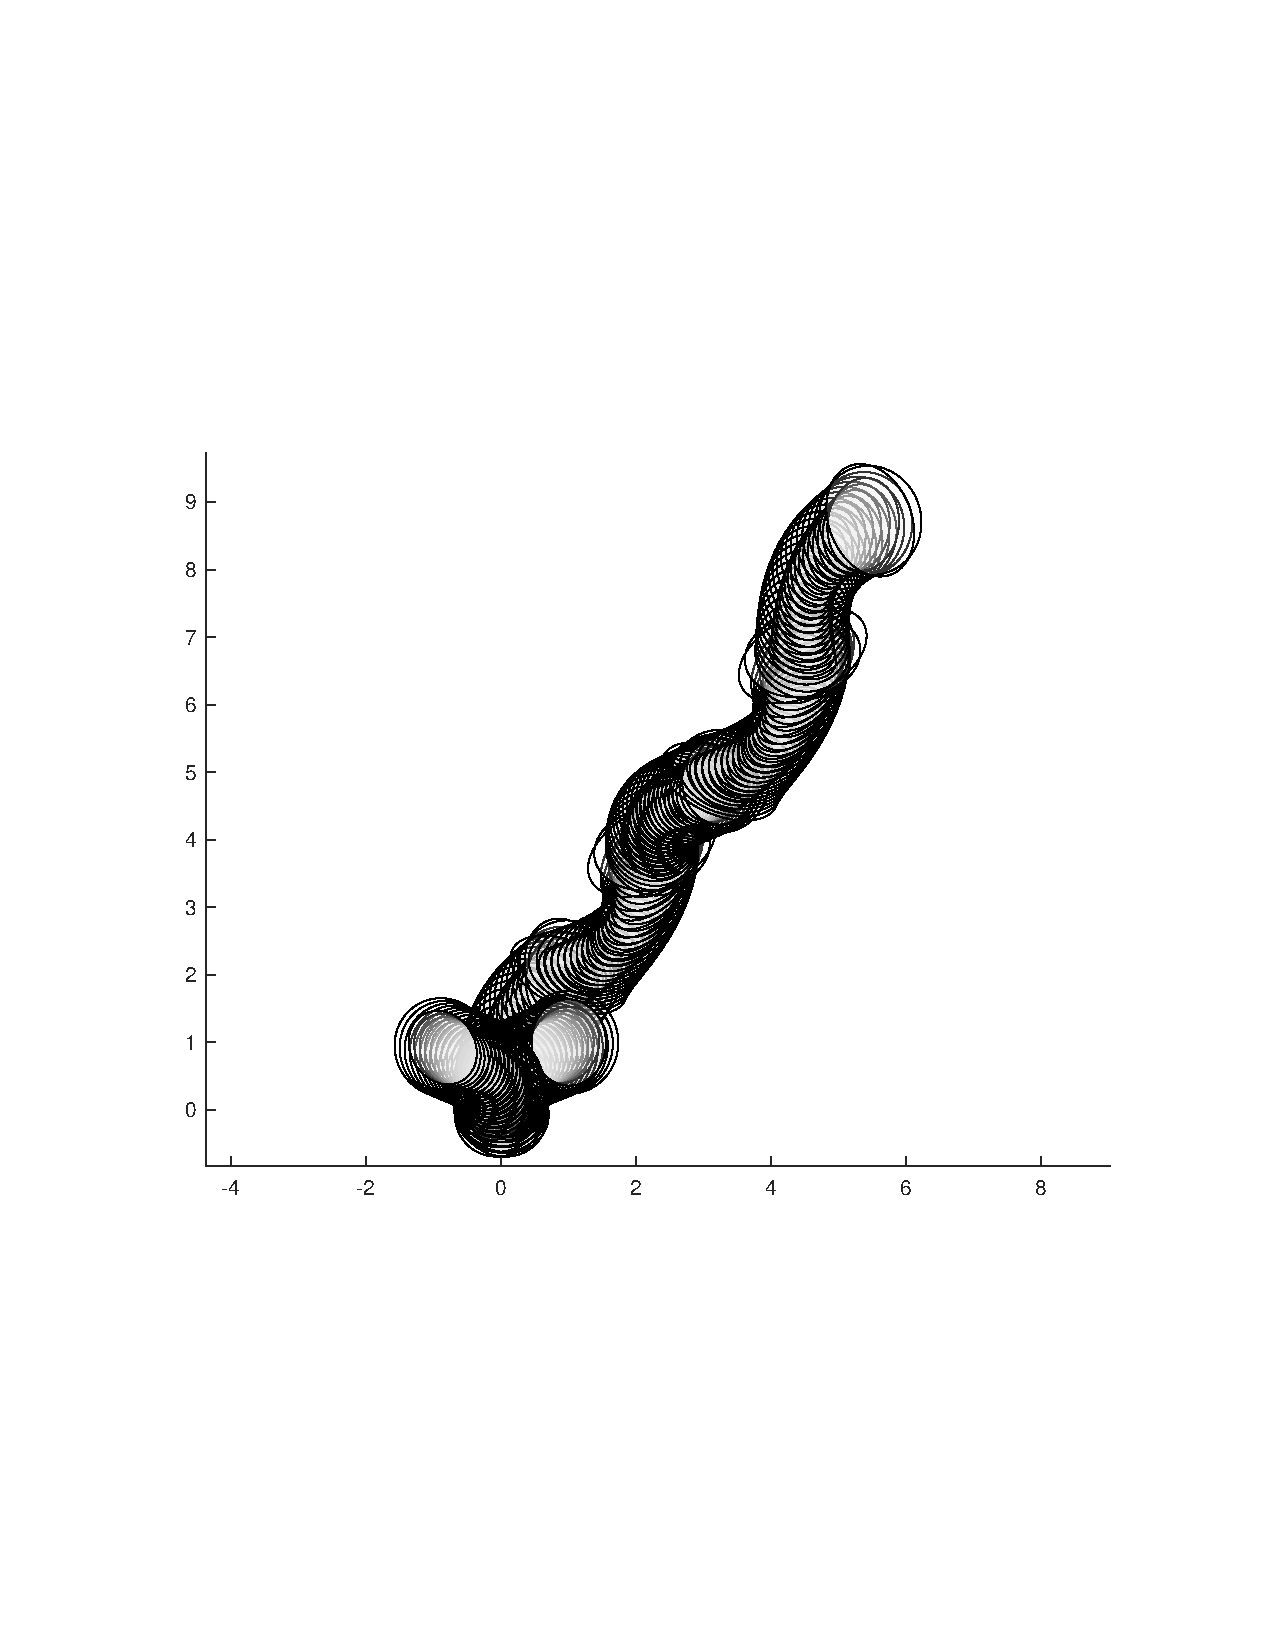
\includegraphics[scale=.5]{figures/method/funnel-tree}
  \caption{Picutred: A tree of funnels built by the \rrtfunnel{} algorithm.}
\end{figure}

The \rrtfunnel{} algorithm is defined as


\begin{algorithm}[H]
  \caption{\rrtfunnel{} algorithm}

  \DontPrintSemicolon

  \KwIn{Initial configuration, \(q_0\)}
  \KwOut{\textit{RRT}-Funnel-graph \(\mathcal{G}\)}

  \SetKwFunction{RandConf}{Sample\_Random\_Configuration}
  \SetKwFunction{NearestVertex}{Find\_Nearest\_Vertex}
  \SetKwFunction{Extend}{Extend}
  \SetKwFunction{AddVertex}{add\_vertex}
  \SetKwFunction{AddEdge}{add\_edge}
  \SetKwFunction{ExtractBranch}{Extract\_Branch}

  \(\mathcal{G}.init(q_0)\)
  \For{\(i \leftarrow 1\) \KwTo \(k\)}{
    \(q_{rand} \leftarrow \) \RandConf{} \;
    \(q_{near} \leftarrow \) \NearestVertex{\(q_{rand}, \mathcal{G}\)}\;
    \(q_{new} \leftarrow \) \Extend{\(q_{near}, q_{rand} \)}\;
    \If{\(q_{new} \in \modelconfigurationspacefree{} \) } {
      \(\mathcal{G}\).\AddVertex{\(q_{new}\)}\;
      \(\mathcal{G}\).\AddEdge{\(q_{near}, q_{new}\)} \;
      \If{\(q_{new} \in \mathcal{X}_{goal}\)}{
        return \ExtractBranch{\(\mathcal{G}\)} \;
      }\;
    }
  }

  \SetKwProg{Def}{def}{:}{end}
  \Def{\RandConf{}}{
    return 0\;
  }
  \Def{\NearestVertex{\(q_{rand}, \mathcal{G}\)}}{
    return 0\;
  }
  \Def{\Extend{\(q_{near}, q_{rand} \)}}{
    return 0\;
  }

  \Def{\ExtractBranch{}}{
    return 0\;
  }

\end{algorithm}